%%%%%%%%%%%%%%%%%%%%%%%%%%%%%%%%%%%%%%%%%%%%%%%%%%%%
%    Canadian AI Latex Template    %
%%%%%%%%%%%%%%%%%%%%%%%%%%%%%%%%%%%%%%%%%%%%%%%%%%%%
\documentclass[10pt]{cai}
\captionsetup{font=small}
\begin{document}
% Editorial staff will replace the following values:
% 1. Conference Year
% 2. Issue number
% 3. Article DOI
\def\conferenceyear{2025}
\volumeheader{38}{0}%{00.000}
\begin{center}

\title{Development of a Reinforcement Learning Enabled Cattle Tracker Prototype}
\maketitle

\thispagestyle{empty}

% Add Authors and Affiliations in the camera ready
% for the double blind review, please leave this section as is 
\begin{tabular}{cc}
First Author\upstairs{\affilone,*}, Second Author\upstairs{\affilone}, Third Author\upstairs{\affilthree}
\\[0.25ex]
{\small \upstairs{\affilone} Affiliation One} \\
{\small \upstairs{\affiltwo} Affiliation Two} \\
{\small \upstairs{\affilthree} Affiliation Three} \\
\end{tabular}
  
% Replace with corresponding author email address
\emails{
  \upstairs{*}corresponding\_author@example.ca 
}
\vspace*{0.2in}
\end{center}

\begin{abstract}
The increasing demand for precision livestock monitoring has led to the development of Internet of Things (IoT)-enabled solutions for real-time tracking and health assessment of cattle. 
In this study, we present the development of a reinforcement learning-enabled cattle tracker prototype designed to optimize power consumption while ensuring continuous data collection and transmission. 
The prototype integrates IoT sensors, solar power collection, and reinforcement learning-based decision-making to dynamically balance data transmission, storage, and energy conservation. 
The reinforcement learning agent autonomously determines the optimal transmission schedule based on power availability, maximizing data efficiency while prolonging battery life. 
The agent is trained on measured prototype data and the reward function is tuned from a Bayesian optimization to maximize the message collection.
Experimental evaluations demonstrate the prototype's capability to sustain long-term operation under real-world environmental constraints. 
The results highlight the feasibility of integrating machine learning with IoT devices for adaptive, energy-efficient cattle monitoring.
Our findings contribute to the broader field of smart agriculture by demonstrating how reinforcement learning can be leveraged to enhance IoT-based livestock management. 
Future work will focus on optimizing the decision-making model for diverse environmental conditions and scaling the system for larger deployments.

\end{abstract}

% add your keywords
\begin{keywords}{Keywords:}
Internet of Things (IoT), Reinforcement Learning, Cattle Monitoring.
\end{keywords}
\copyrightnotice

\section{Introduction}

Timely tracking of free range beef cattle is essential for farmers to assess herd health and monitor animal behaviors. 
Internet of Things (IoT)-based solutions have been developed to replace labor-intensive manual observation with automated, real-time monitoring \cite{unoldIoTBasedCowHealth2020} \cite{yamsaniIoTBasedLivestockMonitoring2024}.
The devices take the form of collars, leg bands, or ear tags and are small, low power, equipped with sensors and communication modules, and have limited communication capabilities, but provide insights into the environment that they are deployed in \cite{unoldIoTBasedCowHealth2020} \cite{moutaouakilDigitalFarmingSurvey2023}.
However, their installation is a time consuming process, making long-term autonomous operation (months), without human intervention, a key requirement.
Power limitations remain another significant challenge, as frequent data transmission depletes battery, necessitrating the design of energy-efficient solutions.
Solar panels can extend battery life, while their effectiveness relys heavily on weather conditions and the cattle's orientation and location.

Reinforcement learning (RL) is a branch of machine learning that allows an agent to learn strategies to maximize a reward.
The agent learns by interacting with the environment and updating its behaviour based on the received rewards for those actions\cite{suttonReinforcementLearningIntroduction2020}.
The combination of reinforcement learning and IoT devices, also called the Artificial intelligence of Things (AIoT), offers a promising alternative by dynamically optimizing energy consumption through adaptive decision-making.
The TinyML paradigm, a subset of AIoT, focuses on machine learning on devices with highly constrained resources and is often limited to inference only\cite{rayReviewTinyMLStateoftheart2022}.
Overall, the addition of intelligence to the device allows it to make better decisions, however, on the other hand the addition of intelligence to the device increases the power consumption of the device.

In this paper, we present a reinforcement learning-enabled cattle tracker prototype that autonomously optimizes power consumption by deciding when to transmit, store, or delay data collection.
The Q-learning-based agent adapting to varying power availability and the device incorporates solar power to extend operational longevity.
Our approach ensures uninterrupted monitoring while balancing energy efficiency and data quality. 
By leveraging RL, the proposed system outperforms static scheduling approaches, allowing for the collection of uninterrupted data, as well as occasionally check in, making it a viable solution for long-term autonomous cattle tracking.

\section{Related Work}
% IoT and Cloud
IoT sensors are faced with (i) limited battery life, (ii) limited processing power, and (iii) limited storage\cite{chenDeepReinforcementLearning2021}.
Model training is computationally expensive so devices that fall under the TinyML paradigm are often limited to inference only\cite{rayReviewTinyMLStateoftheart2022}.
The addition of cloud communication opens the possibility of training the model in the cloud and deploying a new model to the device that adapts to changes in the environment.

%Cattle and IoT
Existing IoT-based cattle monitoring solutions have primarily focused on health tracking, behavior classification, and disease detection using machine learning and sensor networks. 
Studies such as \cite{duttaMOOnitorIoTBased2022} have proposed multi-sensory IoT devices for cattle activity monitoring using XGBoost and Random Forest classifiers. 
\cite{yamsaniIoTBasedLivestockMonitoring2024} introduced an ML-based livestock management system that classifies cattle behavior but does not optimize energy consumption. 
Additionally, \cite{arshadFederatedLearningModel2024} and \cite{iRealTimeCattle2024} have applied LoRa-based IoT solutions and federated learning for disease detection, emphasizing data accuracy over power efficiency.

% Reinforcement Learning
In contrast, our work integrates RL to dynamically optimize power consumption in cattle trackers, ensuring long-term device operation while maintaining data quality. 
Prior studies, such as \cite{hribarUsingDeepQLearning2019}, demonstrated that deep Q-learning could extend IoT device battery life, but their work relies on a network of devices to determine whether correlated sensors should transmit data or save power.
Our system leverages RL-driven decision-making for a single device to balance data transmission, storage, and power conservation, addressing a key limitation in prior research.


\section{System Design and Architecture}

AIoT device design is an iterative process involving simulations, hardware development, measurement, and redeployment
Automation is essential to facilitate rapid development with reduced human intervention.
RL helps this process by allowing the device to adapt to new parameters without the need for manual update of collection strategies.

\subsection{Q-learning}

Central to Q-learning, a widely used RL approach, is the action-value function $Q(S_t, A_t)$, which is the expected cumulative reward of taking action $a$ in state $s$.
The agent approximates the optimal policy by updating the action-value function based on the reward that it receives during training\cite{suttonReinforcementLearningIntroduction2020}:

\begin{equation}
Q^{new}(S_t, A_t) \leftarrow Q(S_t, A_t) + \alpha \left[ R_{t+1} + \gamma \max_{a} Q(S_{t+1}, a) - Q(S_t, A_t) \right]
\end{equation}

where $\alpha$ is the learning rate, $\gamma$ is the discount factor, and $R_{t+1}$ and $S_{t+1}$ is the reward and state after taking action $A_t$ in state $S_{t}$, respectively.

The agent's state consists of time of day $T$, battery power level $p$, and queued message count $m$.
$T$ (discretized into 48 bins) informs the power generation likelihood, $p$ was discretized to 100 levels, and $m$ was discretized to 5 levels to enforce a transmission check every 2.5 hours to prevent data loss.
This resulted in $T\times p \times m = 24,000$ possible states. The agent action space contains three discrete actions: $\mathcal{A}=\{a_0, a_1, a_2\}$, where $a_0=$delay data collection, $a_1=$collect and store data, and $a_2=$collect and transmit data, turning the action-value function into a $24000 \times 3$ table.

A tabular representation for $Q(S_t, A_t)$ was used as it turns the model inference into a table lookup with $O(1)$ complexity.
Deep Q-learning alternatives, which use a neural network to approximate $Q(S_t, A_t)$ require additional on-device compuation and were not considered.
A tabular representation does require larger memory or storage, but can be partially updated from the cloud to reflect new conditions.

The goal of the agent is to maximize the number of messages sent to the cloud and the power level of the device.
It is not trivial to determine the reward values that achieve this goal.
We consider the reward values to be hyperparameters and used a Bayesian optimization framework from the the python \verb|scikit-optimize| package to tune them.
The hyperparameters (Table~\ref{tab:reward_parameters}) show that the most negative reward is for delaying collection. 
The reward for transmitting data also collects the reward per message, which only becomes attractive if there are messages in the queue.

\begin{table}[h]
  \centering
  \caption{Reward function parameters extracted during hyperparameter tuning.}
  \begin{tabular}{l p{8cm} c}
      \toprule
      \textbf{Parameter} & \textbf{Description} & \textbf{Value} \\
      \midrule
      reward\_power\_loss & reward for full discharge of battery & 0.00  \\ 
      reward\_power\_multiplier & reward per power level at every time step & 0.0001  \\ 
      reward\_action\_0 & reward for delaying collection & -1.716 \\ 
      reward\_action\_1 & reward for collecting and storing data & -0.600 \\ 
      reward\_action\_2 & reward for collecting and transmitting data & -1.485 \\ 
      reward\_message\_count & reward for each message at transmission & 0.841 \\ 
      \bottomrule
  \end{tabular}
  \label{tab:reward_parameters}
\end{table}

The agent was trained in a simulated environment with the power consumption and generation numbers collected from the prototype hardware.
At each step, the environment updates the battery level, time of day, and queued messages based on the agent's action.
The 1300 mAh battery (discretized into 100 levels) drains 5.0 mAh per 30 minutes in sleep mode, while transmission and data collection consume 1.6 mAh and 0.1 mAh, respectively.

Solar gain data from 17 June days in Edmonton was averaged into sunny and cloudy profiles, with an 80\% probability of a cloudy day. 
This constraint limited power availability, forcing the agent to optimize message transmission. 
The training process was repeated four times with different seeds for each hyperparameter search iteration. 
Once the optimal hyperparameters were found, the action-value function was exported as an h-file for firmware deployment. 
This automated approach reduced manual effort and effectively optimized reward values.


\subsection{Hardware}
The hardware prototype is shown in figure \ref{fig:prototype} and consists of an Arduino microcontroller, a GPS device, a solar array, a power distribution system, and a battery.
The detailed specifications are shown in table \ref{tab:hardware_inventory}. 
Prototype testing revealed high sleep power consumption (9.9 mA) due to always-on LEDs and integrated components. 
A custom PCB with full component isolation is planned to reduce sleep current to $\mu A$ levels.
An unexpected benefit of high power draw was a faster development cycle, as battery depletion occurred in days rather than weeks.

\begin{table}[h]
  \centering
  \caption{Hardware list for the cattle tracker prototype}
  \begin{tabular}{l p{6.5cm} c}
      \toprule
      \textbf{Hardware} & \textbf{Description} & \textbf{Serial Number} \\
      \midrule
      Arduino MKR WiFi 1010 & WiFi-enabled microcontroller board & ABX00023 \\
      Arduino MKR GPS Shield & Integrated GPS module & ASX00017 \\
      DFRobot Solar Power Manager & Power dsitribution board & TPX00046 \\
      Solar Panel & 75x100x2.9 mm panel, 1W output & TPX00181 \\
      Sparkfun Fuel Gage & Analog sensor for power measurement & 1568-1273-ND \\
      LiPo Battery & 3.7V, 2000mAh capacity & 2528 \\
      \bottomrule
  \end{tabular}
  \label{tab:hardware_inventory}
\end{table}

\begin{figure}[h]
  \centering
  \begin{subfigure}[t]{0.48\textwidth}  % Align top
      \centering
      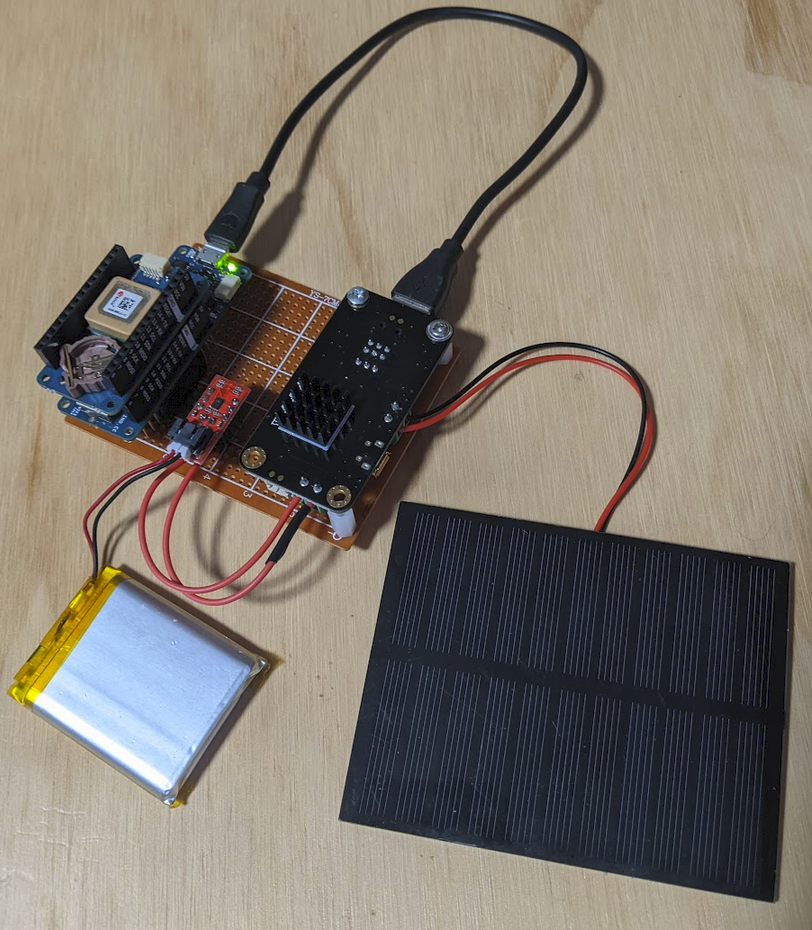
\includegraphics[height=6cm, keepaspectratio]{./figs/prototype.png}
      \put(-170,160){\scriptsize \textbf{(A)}}  % Adjust position as needed
      \label{fig:prototype_real}
  \end{subfigure}
  \hspace{2mm}  % Reduce space between figures
  \begin{subfigure}[t]{0.48\textwidth}  % Align top
      \centering
      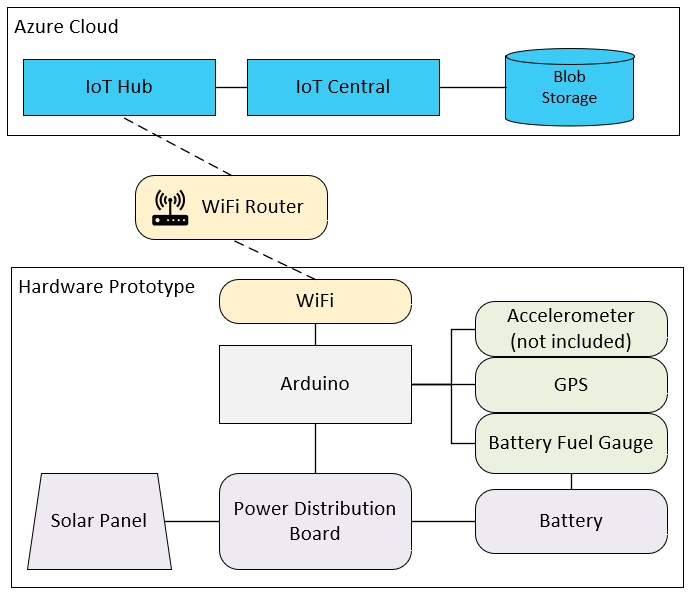
\includegraphics[height=6cm, keepaspectratio]{./figs/prototype_diagram.png}
      \put(-215,160){\scriptsize \textbf{(B)}}  % Adjust position as needed
      \label{fig:prototype_diagram}
  \end{subfigure}
  \caption{(A) Physical prototype with hardware components. (B) System architecture diagram illustrating data processing and power management.}
  \label{fig:prototype}
\end{figure}


\subsection{Firmware}
The prototype firmware, written in Arduino C++, handles sensor data collection, decision-making, and cloud transmission (see Figure~\ref{fig:prototype} B). 
The main loop runs every 30 minutes, alternating between sleep mode and decision-making.
At each decision point, the device reads the time, battery level, and queued messages, retrieves a recommended action, and executes it.
Due to memory constraints, only the highest-value action per state was stored, reducing the policy table size. 
The policy was bit-shifted into and array of 32-bit integers for efficient storage in memory.


\subsection{Cloud}
The prototype transmits data to Azure IoT Hub, which integrates with IoT Central for dashboarding and Blob Storage for data retention (see Figure~\ref{fig:prototype} B). 
IoT Central supports device registration, dashboard creation, and digital twins, enabling remote monitoring and state updates.
The cloud facilitates two-way communication, allowing the device to receive policy updates for potential seasonal changes or location-specific solar gain variations.


\section{Results}

\subsection{Simulation Training Results}
To evaluate the effectiveness of the reinforcement learning agent, we compare it to a baseline collection strategy that alternates between data collection and transmission, sending data once per hour. 
This represents a simple, fixed scheduling approach.
Table~\ref{tab:agent_comparison} shows that the RL agent reduces transmissions, conserving power while increasing collection actions, leading to a higher message count (+4.3\%) and a more sustainable average power level (76 vs. 34).
The trained agent optimized collection-to-transmission behavior, performing 2.12 collection actions per transmission, compared to the 1:1 fixed schedule of the baseline. 
This suggests the agent learned an adaptive strategy, balancing energy efficiency with message throughput.


\begin{table}[h]
  \centering
  \caption{Comparison of baseline agent and RL agent}
  \begin{tabular}{lcc}
      \toprule
      & Baseline Agent & RL Agent \\
      \midrule
      Transmission Actions & 480 & 308 \\
      Collection Actions & 480 & 652 \\
      Sleep Actions & 0 & 0 \\
      Avg. Message Count & 756.5 & 789.5 \\
      Avg. Power Level & 34 & 76 \\
      \bottomrule
  \end{tabular}
  \label{tab:agent_comparison}
\end{table}


\subsection{Deployment Results}
The trained agent was deployed on the prototype hardware in an indoor environment without power generation for a 9-day evaluation period, with occasional manual charging to ensure continuous operation.  
This test assessed the agent’s long-term decision-making performance in real hardware and validated its ability to operate under realistic power constraints. The results are shown in Figure~\ref{fig:prototype_result}.
During the test, the hardware experienced several outages, the longest lasting 3.6 hours on 2024-10-07.  
The agent maintained an average collection-to-transmission ratio of 2.18, which closely matches the simulation results.  

\begin{figure}[h]
  \centering
  \begin{subfigure}{0.48\textwidth}
      \centering
      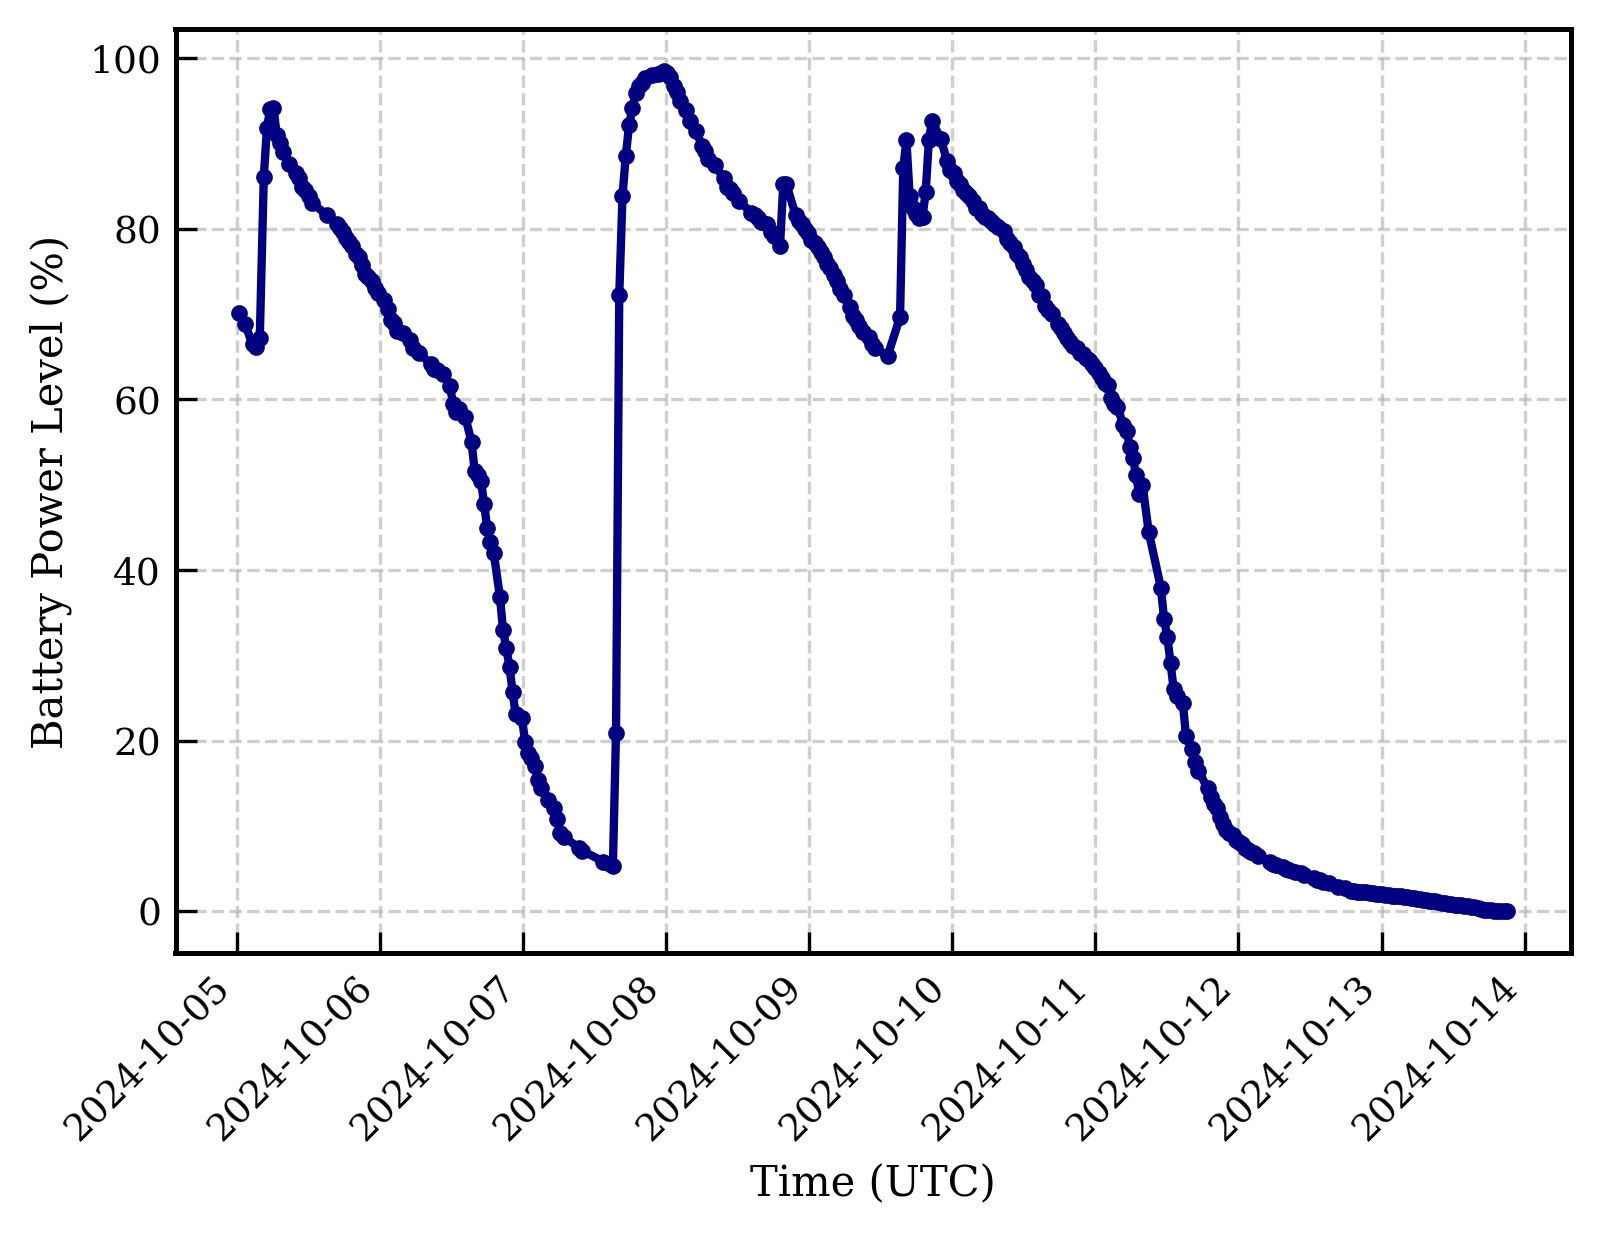
\includegraphics[width=\linewidth]{figs/prototype_power_level.png}
      \put(-195,138){\scriptsize \textbf{(A)}}  % Adjust position
      \label{fig:prototype_power}
  \end{subfigure}
  \hfill
  \begin{subfigure}{0.48\textwidth}
      \centering
      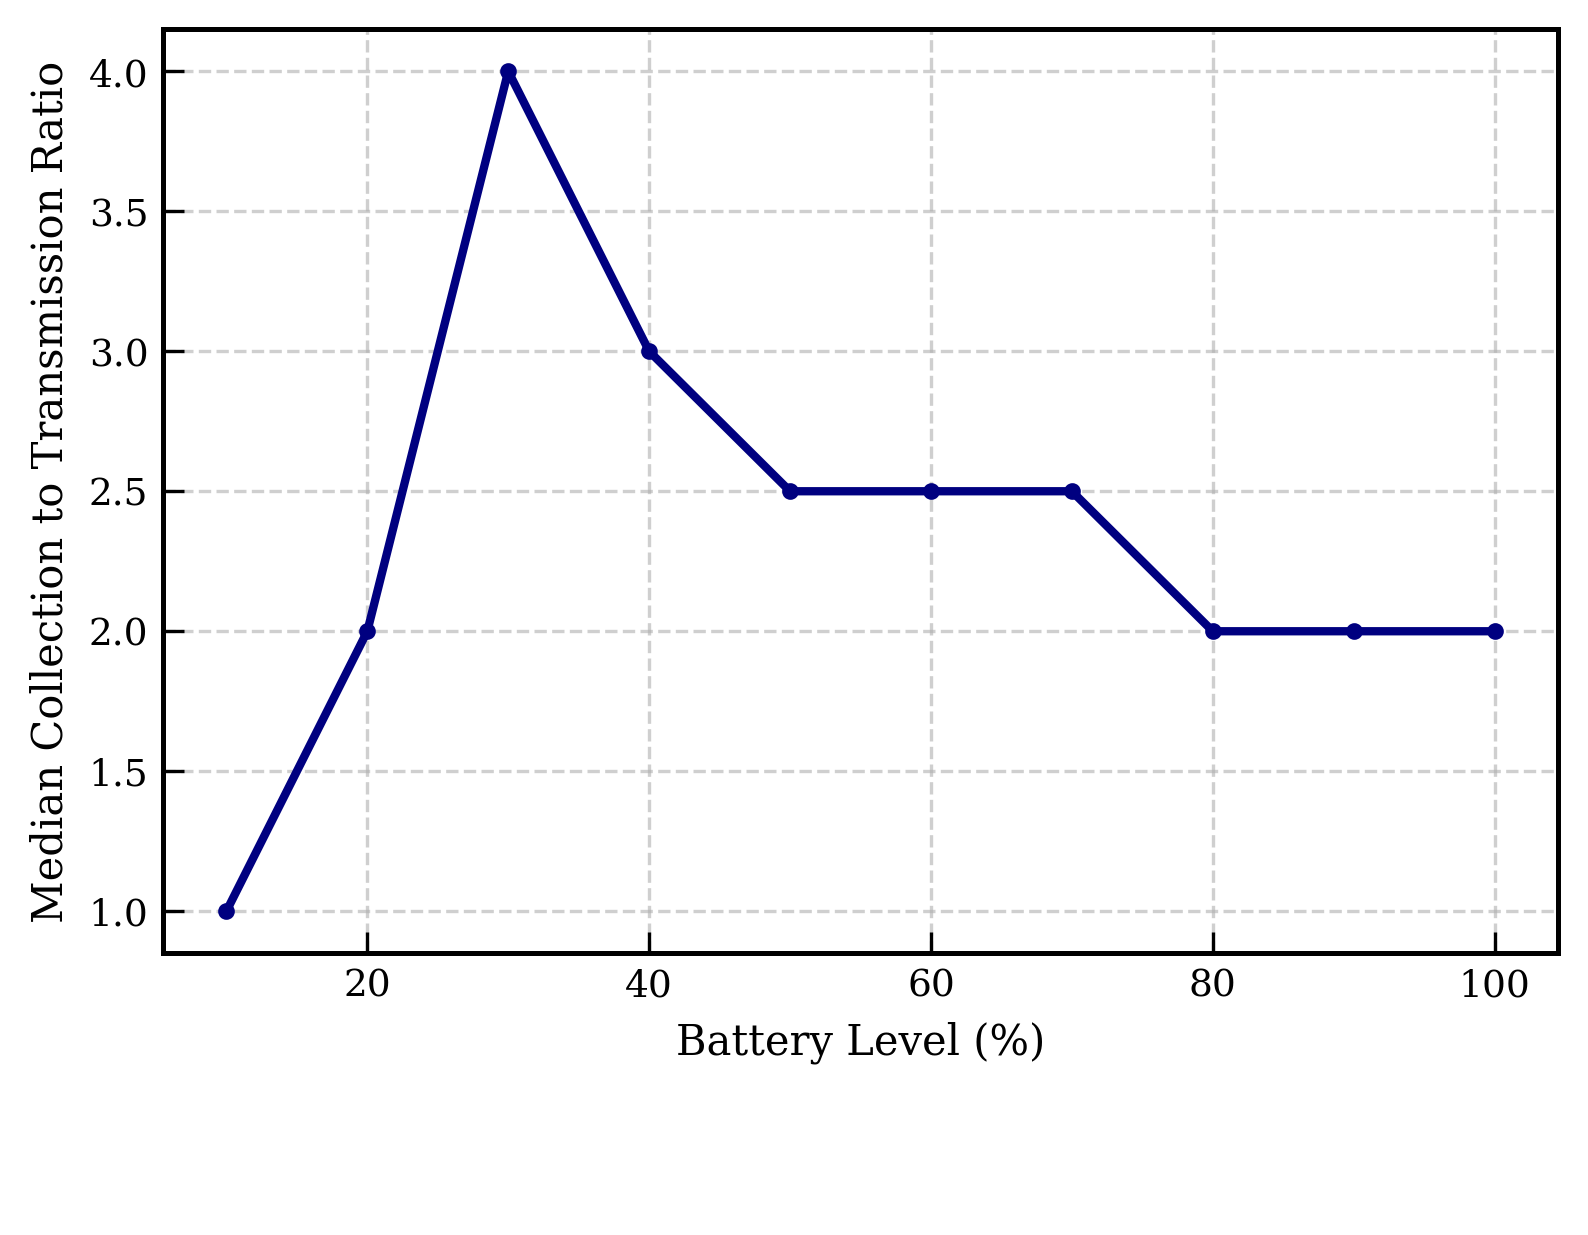
\includegraphics[width=\linewidth]{figs/battery_level_vs_collection_ratio.png}
      \put(-195,138){\scriptsize \textbf{(B)}}  % Adjust position
      \label{fig:battery_vs_collection}
  \end{subfigure}
  \caption{(A) Nonlinear power level discharge over a 9-day period. (B) Learned agent strategy adapting to varying power levels.}
  \label{fig:prototype_result}
\end{figure}

Figure~\ref{fig:prototype_result}\subref{fig:battery_vs_collection}A illustrates the nonlinear battery discharge curve observed over the 9-day period.  
The discharge rate during sleeping is relatively constant and the nonlinearity is a result of the mapping function of voltage to remaining capacity.
While sleep mode consumption remains constant, the voltage-to-capacity mapping introduces nonlinearity, making it difficult for the agent to accurately predict future battery levels at low charge states.

Figure~\ref{fig:prototype_result}\subref{fig:battery_vs_collection}B shows the agent's adaptive strategy under varying power levels.
The agent alternates between collection and transmission at full charge, prioritizes storage with a 4:1 collection-to-transmission ratio at 30\% power, and transmits every collected message at low power which accelerates battery drain.
Messages are stored in volatile memory so the queue is lost when the battery is fully discharged.
The agent learned to transmit every time to prevent data loss at low power levels.
This revealed a short-coming of the prototype and future iterations will store the queue in non-volatile memory to prevent data loss.

\section{Conclusion}
In this study, we developed a Q-learning-enabled cattle tracker that optimizes power consumption while ensuring efficient data collection and transmission. 
The device dynamically adjusts its strategy based on energy availability, time of day, and message queue length, improving battery life and efficiency. 
By integrating solar power with adaptive decision-making, the prototype offers a viable solution for long-term autonomous tracking. 
Future work will focus on hardware optimizations, including low-power components and a custom PCB to enhance reliability and longevity. 
Additionally, we aim to increase the message queue length, improve the reward function to account for the age of the messages, and incorporate non-volatile memory storage.


\section*{Acknowledgements}

% All references should be stored in the file "references.bib".
% That call to use that file is in "cai.cls". 
% Please do not modify anything below this line.
\printbibliography[heading=subbibintoc]

\end{document}
